%! app: TODOapp
%! outcome: TODOoutcome

Draw a logic circuit that implements fixed-width 2 binary addition:
\begin{itemize}
\item Inputs  $x_0, y_0, x_1, y_1$ represent $(x_1  x_0)_{2,2}$ and $(y_1 y_0)_{2,2}$
\item Outputs  $z_0, z_1, z_2$ represent $(z_2  z_1 z_0)_{2,3} = (x_1  x_0)_{2,2} + (y_1 y_0)_{2,2}$ (may require up to width  $3$)
\end{itemize}

{\it First approach}: half-adder for each column, then combine carry from right column with sum of left column

\vfill



Write expressions for the circuit output values in terms of input values:

%\vspace{-10pt}

$z_0 = \underline{\phantom{x_0 \oplus y_0\hspace{3in}}}$

%\vspace{-10pt}

$z_1 = \underline{\phantom{(x_1 \oplus y_1) \oplus c_0}\hspace{2.5in}}$ \phantom{where $c_0 = x_0 \land y_0$}

%\vspace{-10pt}

$z_2 = \underline{\phantom{(c_0 \land (x_1 \oplus y_1)) \oplus c_1}\hspace{2in}}$ \phantom{where $c_1 = x_1 \land y_1$}\\

{\it Second approach}: for middle column, first add carry from right column to $x_1$, then add result to $y_1$

\vfill


Write expressions for the circuit output values in terms of input values:

%\vspace{-10pt}

$z_0 = \underline{\phantom{x_0 \oplus y_0}\hspace{3in}}$

%\vspace{-10pt}

$z_1 = \underline{ \phantom{(c_0 \oplus x_1) \oplus y_1}\hspace{2.4in}}$ \phantom{where $c_0 = x_0 \land y_0$}

%\vspace{-10pt}

$z_2 = \underline{\phantom{(c_0 \land x_1) \oplus ((c_0 \oplus x_1)\land y_1)}\hspace{1.5in}}$\\

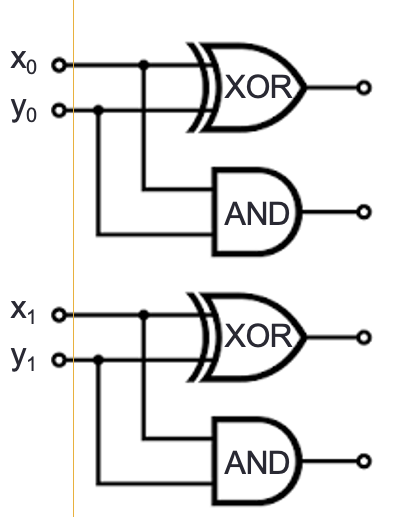
\includegraphics[width=1.7in]{../../resources/images/width-2-adder.png}
\vspace{100pt}

{\it Extra example} Describe how to generalize this addition circuit for larger width inputs.

